

30 minutes of simulations (3x10 minute turulent seeds) performed per wind speed, U = 4, 6, ..., 26 m/s. Normal turbulence model. $f_{1p}$ controller described in previous section is used. Includes effects of tower flexibility, tower shadow, wind shear (power law) and turbulence.
\subsection{Equivalent Load Reduction}


Figure \ref{fig:Spectra_CL} compares the predicted tip deflection spectra (black dotted line) with the simulated spectra (red line). It was found that the predictions fit quite closely with the simulated output. 
\begin{figure}[H]
        \centering
        \begin{subfigure}[b]{0.48\textwidth}
            \centering
            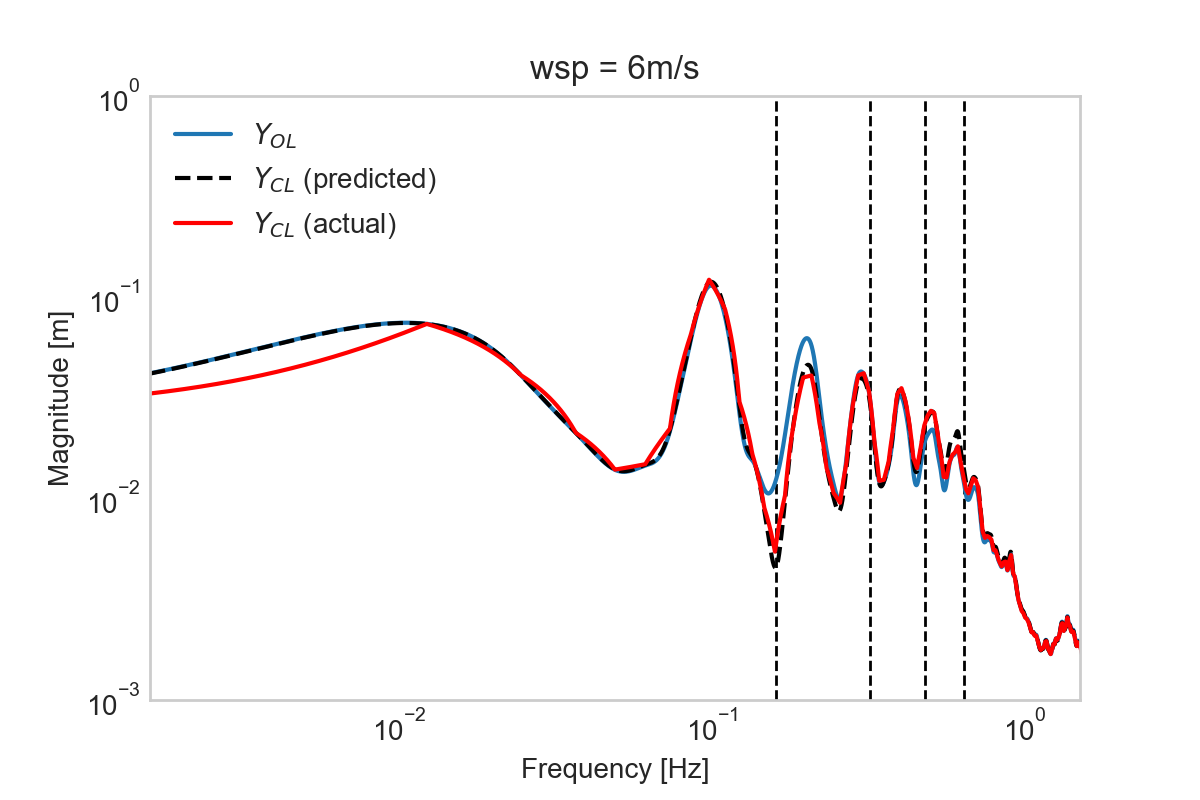
\includegraphics[width=\textwidth]{ipc04_TipDeflection_Spectrum_6.png}
            \caption[Network2]%
            {{\small a}}    
            \label{fig:mean and std of net14}
        \end{subfigure}
        \hfill
        \begin{subfigure}[b]{0.48\textwidth}  
            \centering 
            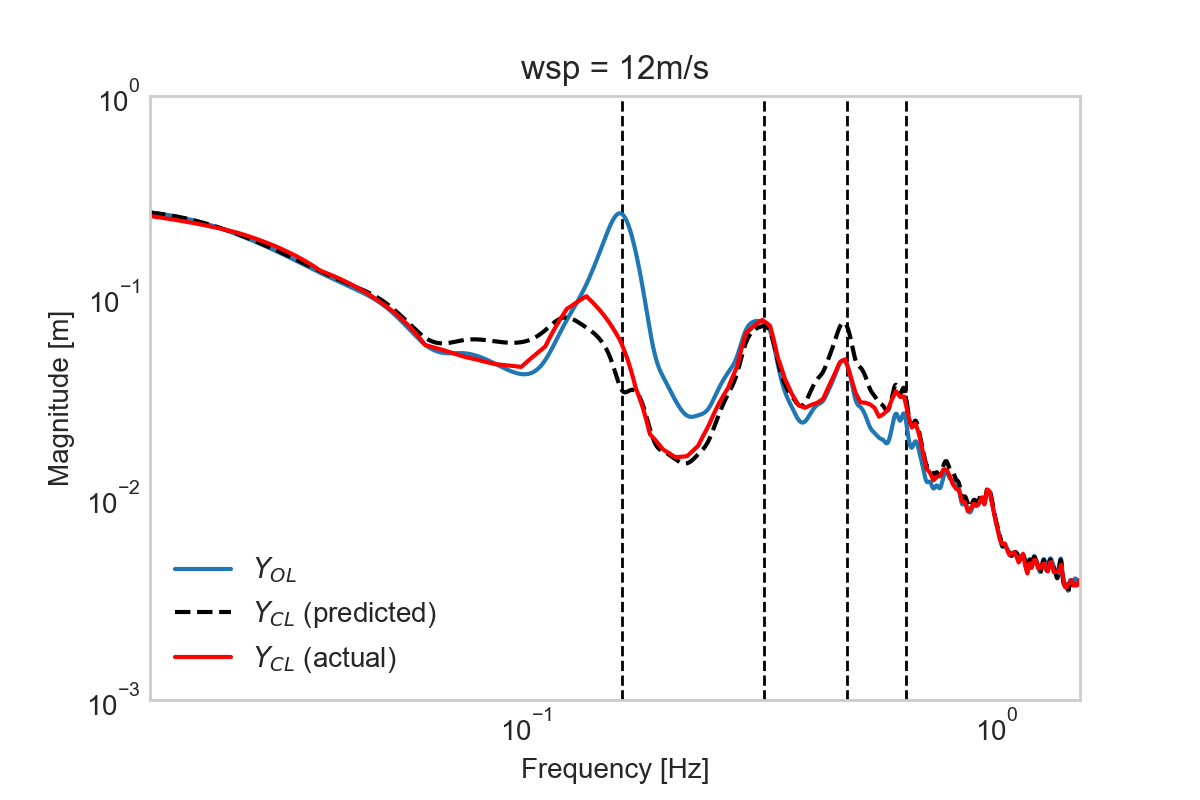
\includegraphics[width=\textwidth]{ipc04_TipDeflection_Spectrum_12.png}
            \caption[]%
            {{\small a}}    
            \label{fig:mean and std of net24}
        \end{subfigure}
        \vskip\baselineskip
        \begin{subfigure}[b]{0.48\textwidth}   
            \centering 
            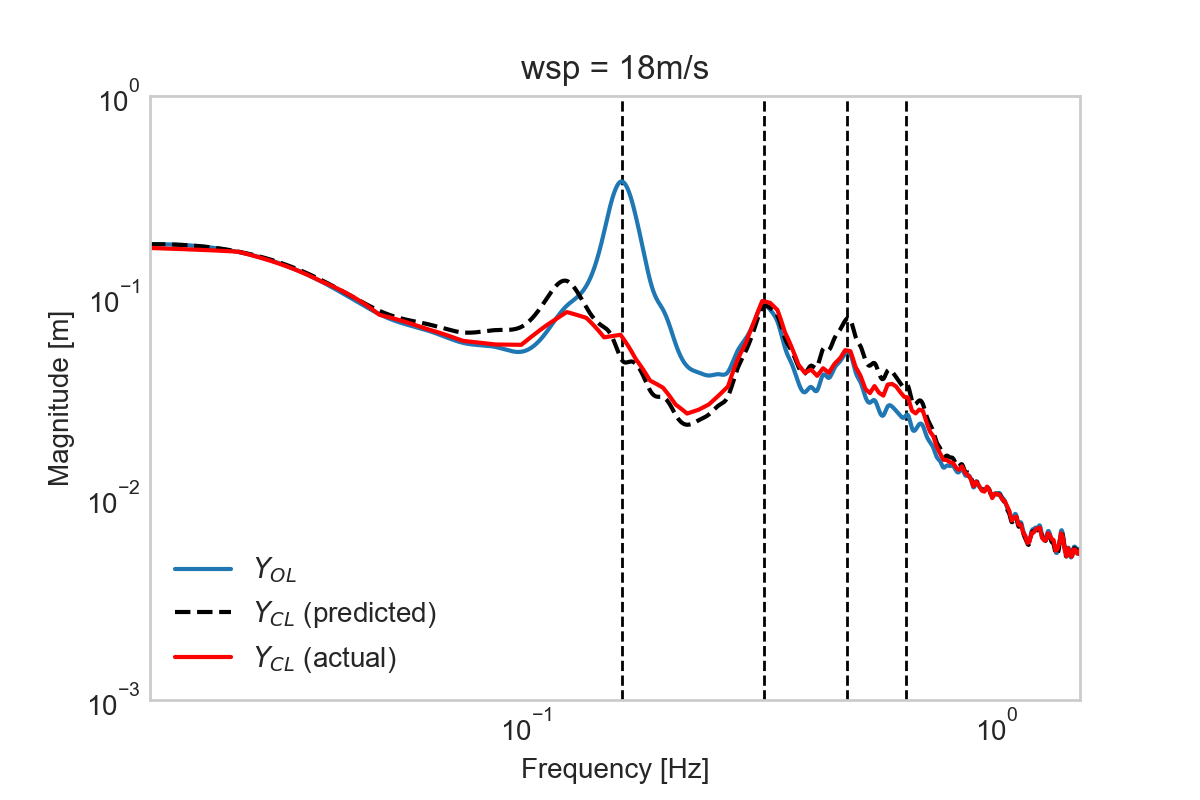
\includegraphics[width=\textwidth]{ipc04_TipDeflection_Spectrum_18.png}
            \caption[]%
            {{\small a}}    
            \label{fig:mean and std of net34}
        \end{subfigure}
        \quad
        \begin{subfigure}[b]{0.48\textwidth}   
            \centering 
            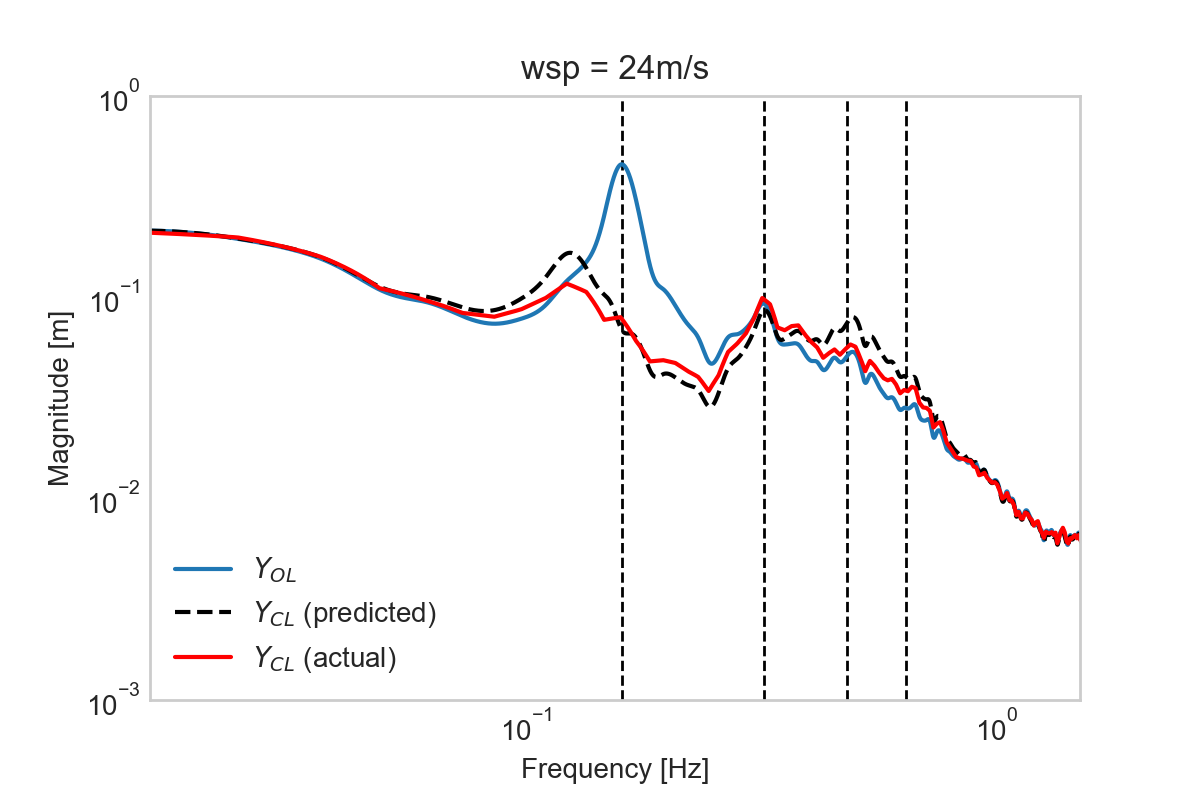
\includegraphics[width=\textwidth]{ipc04_TipDeflection_Spectrum_24.png}
            \caption[]%
            {{\small a}}    
            \label{fig:mean and std of net44}
        \end{subfigure}
        \caption[adsf ]
        {\small asdf} 
        \label{fig:Spectra_CL}
    \end{figure}
To visualise the level of amplification and attenuation at each frequency, Figure \ref{fig:ipc04_SpectralContour} shows the relative spectra as a function of wind speed as a contour plot. Darker regions represent signal attenuation, whereas lighter regions represent signal amplfication. As expected, the controller attenuates tip deflection signal at $f_{1p}$, and encounters slight amplification at $f_{3p}$ and $f_{4p}$ as predicted by the sensitivity function of the modelled feedback loop. The controller underperforms below rated wind speed (~11m/s) as the controller is designed to attenuate frequency components at rated rotor speed. Therefore, in the torque control region where the rotor speed varies, the controller underperforms.
\myFigure[]{ipc04_SpectralContour}{}{fig:ipc04_SpectralContour}   

As predicted, the flapwise blade root bending moment equivalent loads are significantly attenuated above rated wind speed as shown in Figure \ref{fig:ipc04_FatigueLoads_RBM1} at wind speeds above rated. 
\myFigure[]{ipc04_FatigueLoads_RBM1}{}{fig:ipc04_FatigueLoads_RBM1}

The lifetime equivalent loads are calculated for various components and displayed in Figure \ref{ipc04_Lifetime_Req}. Blade flapwise bending moment experiences a 20\% reduction in lifetime equivalent loads. The edgewise loads remain unchanged as expected, and the main bearing experiences a slight increase in loads. This increase can be attributed to the slight amplification in the 4p loads as a result of the control design. The 4p blade loads are transformed to 3p in the fixed fram of reference.
\myFigure[]{ipc04_Lifetime_Req}{}{fig:ipc04_Lifetime_Req}


\subsection{Pitching Limits}
\subsubsection{Pitch Travel}
\subsubsection{Pitch Rate}

\subsection{Influence on Power Output}
Influence of tip deflection control has negligible impact on power output. The distribution of electrical power output with and without tip deflection control is displayed in a violin plot for each wind speed in Figure \ref{fig:ipc04_Power}. Not only are the mean and standard deviation. todo: show a time series as well.
\myFigure[]{ipc04_Power.png}{}{fig:ipc04_Power}
